En esta sección se mostrarán diferentes artículos de investigación y tesis que tratan sobre diversas técnicas y enfoques utilizados para enfrentar problemas similares a los abordados en esta tesis. Además, se incluye un cuadro resumen (véase Anexo \ref{A:table}) con la información presentada en esta sección.


\subsection{Automated recognition of optical image based potato leaf blight diseases using deep learning \citep*{CHAKRABORTY2022101781}}

\citeauthor{CHAKRABORTY2022101781} realizó un artículo de investigación el cual fue publicado en la revista «Physiological and Molecular Plant Pathology» en el año 2022. 
Este fue titulado \citetitle{CHAKRABORTY2022101781} la cual traducida al español significa «Reconocimiento automatizado de enfermedades del tizón de la hoja de la papa basado en imágenes ópticas mediante aprendizaje profundo». La investigación sostiene que el Tizón tardío se presenta como manchas en las hojas de la papa y que para su detección los agricultores sospechan de la patología lo que arriesga los cultivos debido a esta subjetividad y enorme consumo de tiempo. Asimismo, el trabajo explora diferentes recientes modelos de Deep Learning, los cuales los compara con técnicas existentes. 

\subsubsection{Planteamiento del Problema y objetivo }
El artículo aborda la papa como uno de los alimentos más consumidos a nivel mundial, el cual es un elemento relante en la dieta dieria de 1.5 mil millones de personas, pero que se ve afectado por varias patologías. Se plantea que una de las temidas es el Tizón tardío, la cual afecta el rendimiento de producción del tubérculo. Por eso, se requiere una detección temprana para implementar las estrategias de maneja eficaces. Sin embargo, las práticas convencionales para su dignóstico, como la inspección visual, son subjetivos y demandan enorme cantidad de tiempo. Por lo tanto, el artículo plantea que se necesita modelos computacionales avanzados para su clasificación temprana de estas enfermedades, para implementar una gestión y el control de las mismas en la papa. Los principales objetivos son explorar y entrenar modelos de aprendizaje profundo, identificar el modelo de mejor desempeño, optimizar el modelo seleccionado, comparar el modelo propuesto con técnicas existentes y proveer una solución práctica y efeciente.

\subsubsection{Fundamento Teórico usado por el Autor}
El autor planteó emplear recientes modelos de Deep Learning, los principales modelos que utilizó fueron VGG16, VGG19, ResNet50 y MobileNet utilizando imágenes ópticas de hojas de papa del conjunto de datos PlantVillage.



\subsubsection{Metodología empleada por los autores}
La metodología empleada por el autor, para la creación de su chatbot consiste en 6 pasos: 

\begin{figure}[h]
	\begin{center}
		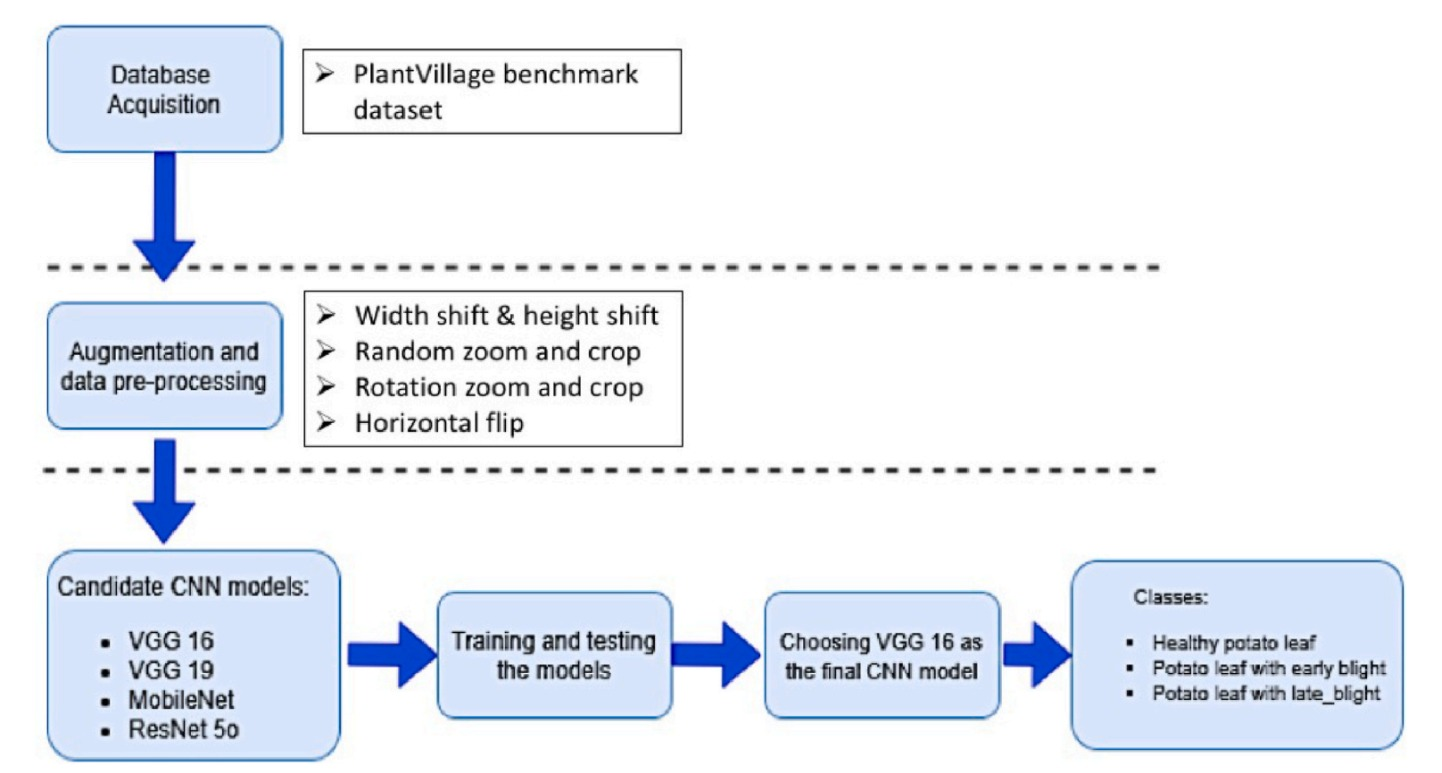
\includegraphics[width=1\textwidth]{2/figures/ant1.jpeg}
		\caption{Metodología propuesta para el modelo (\cite{CHAKRABORTY2022101781})}
	\end{center}
\end{figure}

\begin{enumerate}
	\item Se adquirió la base de datos de imágenes del conjunto de datos PlantVillage, del cual solo extrajo imágenes de hoja de papa.
	\item Realizaron un preprocesamiento de imágenes donde usaron las técnicas de Cambio de ancho, Cambio de Largo, Zoom y recorte aleatorios, Zoom y recortes rotativos y Giro horizontal
	\item Los CNN candidatos fueron  VGG16, VGG19, ResNet50 y MobileNet
	\item Entrenamiento y testeo de los modelos.
	\item Se eligió VGG16 como modelo fianl
	\item Las clases que el modelo clasificaba son, Hoja de papa sana, Hoja de papa con Tizon temprano, Hoja de papa con Tizon tardío
\end{enumerate}

\subsubsection{Resultados obtenidos}



En el paper, cuando se evaluan las distintas técnicas de CNN a considerar, la que sobresale y tiene un mayor desempeño logrando un accuracy promedio del 92.69\%. Es por eso, que se tunea y se escoge como la técnica principal para el desarrollo del modelo final, obteniendo un accuracy promedio del 97.89\%. 

\begin{figure}[H]
	\begin{center}
		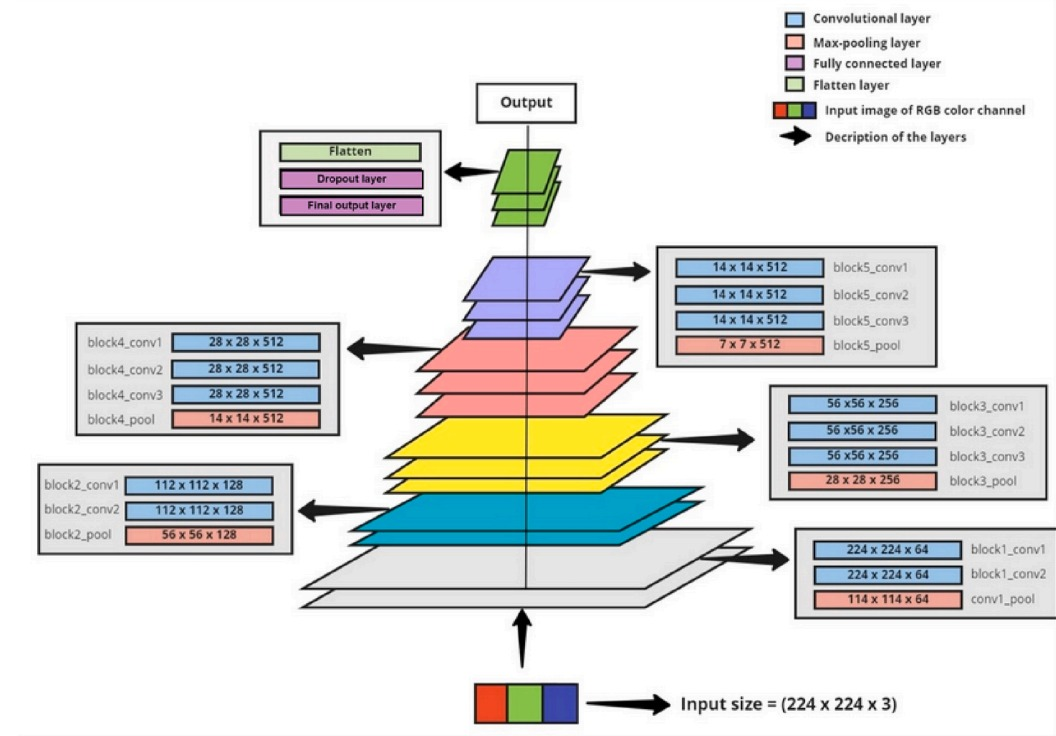
\includegraphics[width=0.8\textwidth]{2/figures/ant1.2.jpeg}
		\caption{Arquitectura del modelo ajustado propuesto de VGG16, muestra las disntitas capas (convolucion). Tambien, se mencionana los respectivos tamaños del filtro convolucional  (\cite{CHAKRABORTY2022101781})}
	\end{center}
\end{figure}

%%%%%%%%%%%%%%%%%%%%%%%%%%%%%%%%%%%%%%%%%%%%%%%%%%%%%%%%%%%%%%%%%%%%%%%%%%%%%%%%%%%%%%%%%%%%%%%%%%%%%%%%%%%%%%%%%%%%%%%%%%%%

\subsection{Research and Validation of Potato Late Blight Detection Method Based on Deep Learning \citep*{antecedente2}}
\citeauthor{antecedente2} realizó este trabajo publicado en la revista Agronomy, para la sección de Precision and Digital Agriculture.
Este fue titulado \citetitle{antecedente2} la cual traducida al español significa «Investigación y validación del método de detección del tizón tardío de la papa basado en aprendizaje profundo». La investigación nos dice que el Tizón tardío puede llevar al fracaso total del cultivo papa. Asimismo, construyeron un total de siete categorías de conjuntos de datos de enfermedades de las hojas de papa en fondos simples y complejos. Finalmente, la investigacion se introduce en diferentes modelos de Deep Learning en distantas versiones.

\subsubsection{Planteamiento del Problema y objetivo }
El trabajo discute sobre el Tizón tardío como enfermedad muy grave para los cultivos de papa. Esta pone en riesgo el total del cultivo, además que los métodos tradicionales como la detección basada en la inspección visual suele ser subjetivo y demora tiempo. Asimismo, los sistemas de detección actuales suelen ser ineficientes debido a la varibilida de luminosidad y el sombreado de las hojas. Es crucial desarrollar un modelo de detección automatizada que pueda superar estas limitaciones, permitiendo una monitorización y prevención temprana del tizón tardío de la papa. El objetivo de este estudio es desarrollar y optimizar un modelo de aprendizaje profundo para la detección del tizón tardío en hojas de papa, que sea altamente preciso y rápido en su inferencia, y que pueda ser implementado en dispositivos móviles para la monitorización automática y la alerta temprana de enfermedades en cultivos. Para alcanzar este objetivo, se plantean las siguientes metas específicas: Lograr una clasificación detallada de enfermedades, Opitmizar el modelo base elegido, Evaluar la viabilidad y efectivdad del modelo en hardware.

\subsubsection{Fundamento Teórico usado por el Autor}

El autor planteó utilizar modelos de Deep Learning, se enfocó en modelos de ligeros y eficientes estos con el fin de implantar el modelo en un dispositivo móvil. Las técnicas que utilizó fueron MobileNet, ShuffleNet, GhostNet, and SqueezeNet pre-trained models usando imágenes de hojas de papa de los conjuntos de dato Plant Village y AI Challenger 2018. 

\begin{figure}[H]
	\begin{center}
		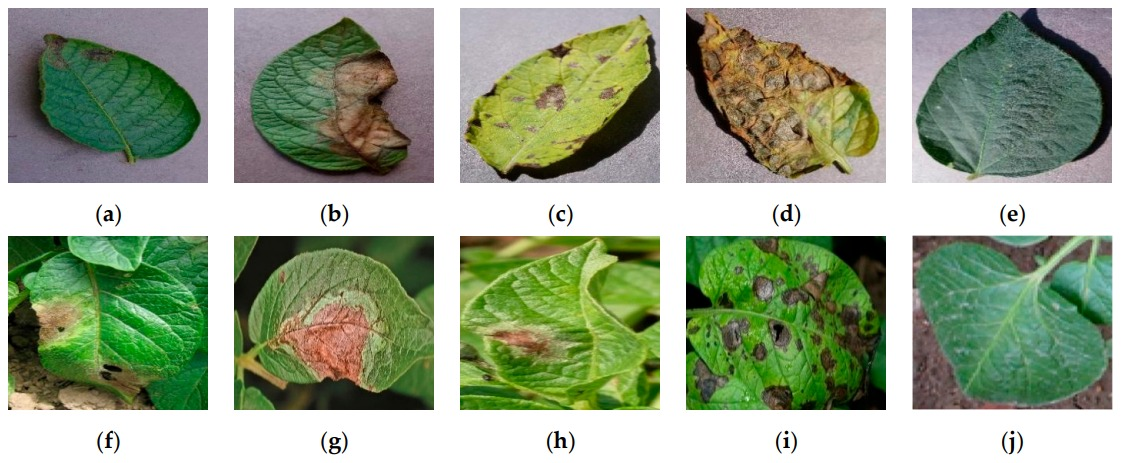
\includegraphics[width=0.6\textwidth]{2/figures/ant2.jpeg}
		\caption{ (a) Etapas tempranas de la hoja con tizón tardío en un contexto único. (b) Etapas finales de la hoja con tizón tardío en un contexto único. (c) Etapas tempranas de la hoja con tizón temprano en un contexto único. (d) Etapas finales de la hoja con tizón temprano en un contexto único. (e) Hoja sana en un contexto único. (f) Etapas tempranas de la hoja con tizón tardío en un contexto natural. (g) Etapas finales de la hoja con tizón tardío en un contexto natural. (h) Etapas tempranas de la hoja con tizón temprano en un contexto natural. (i) Etapas finales de la hoja con tizón temprano en un contexto natural. (j) Hoja sana en un contexto natural. (\cite{antecedente2})}
	\end{center}
\end{figure}


\subsubsection{Metodología empleada por los autores}
La metodología empleada por el autor, para la creación de su modelo final de clasifacion es el siguiente:
 
\begin{figure}[H]
	\begin{center}
		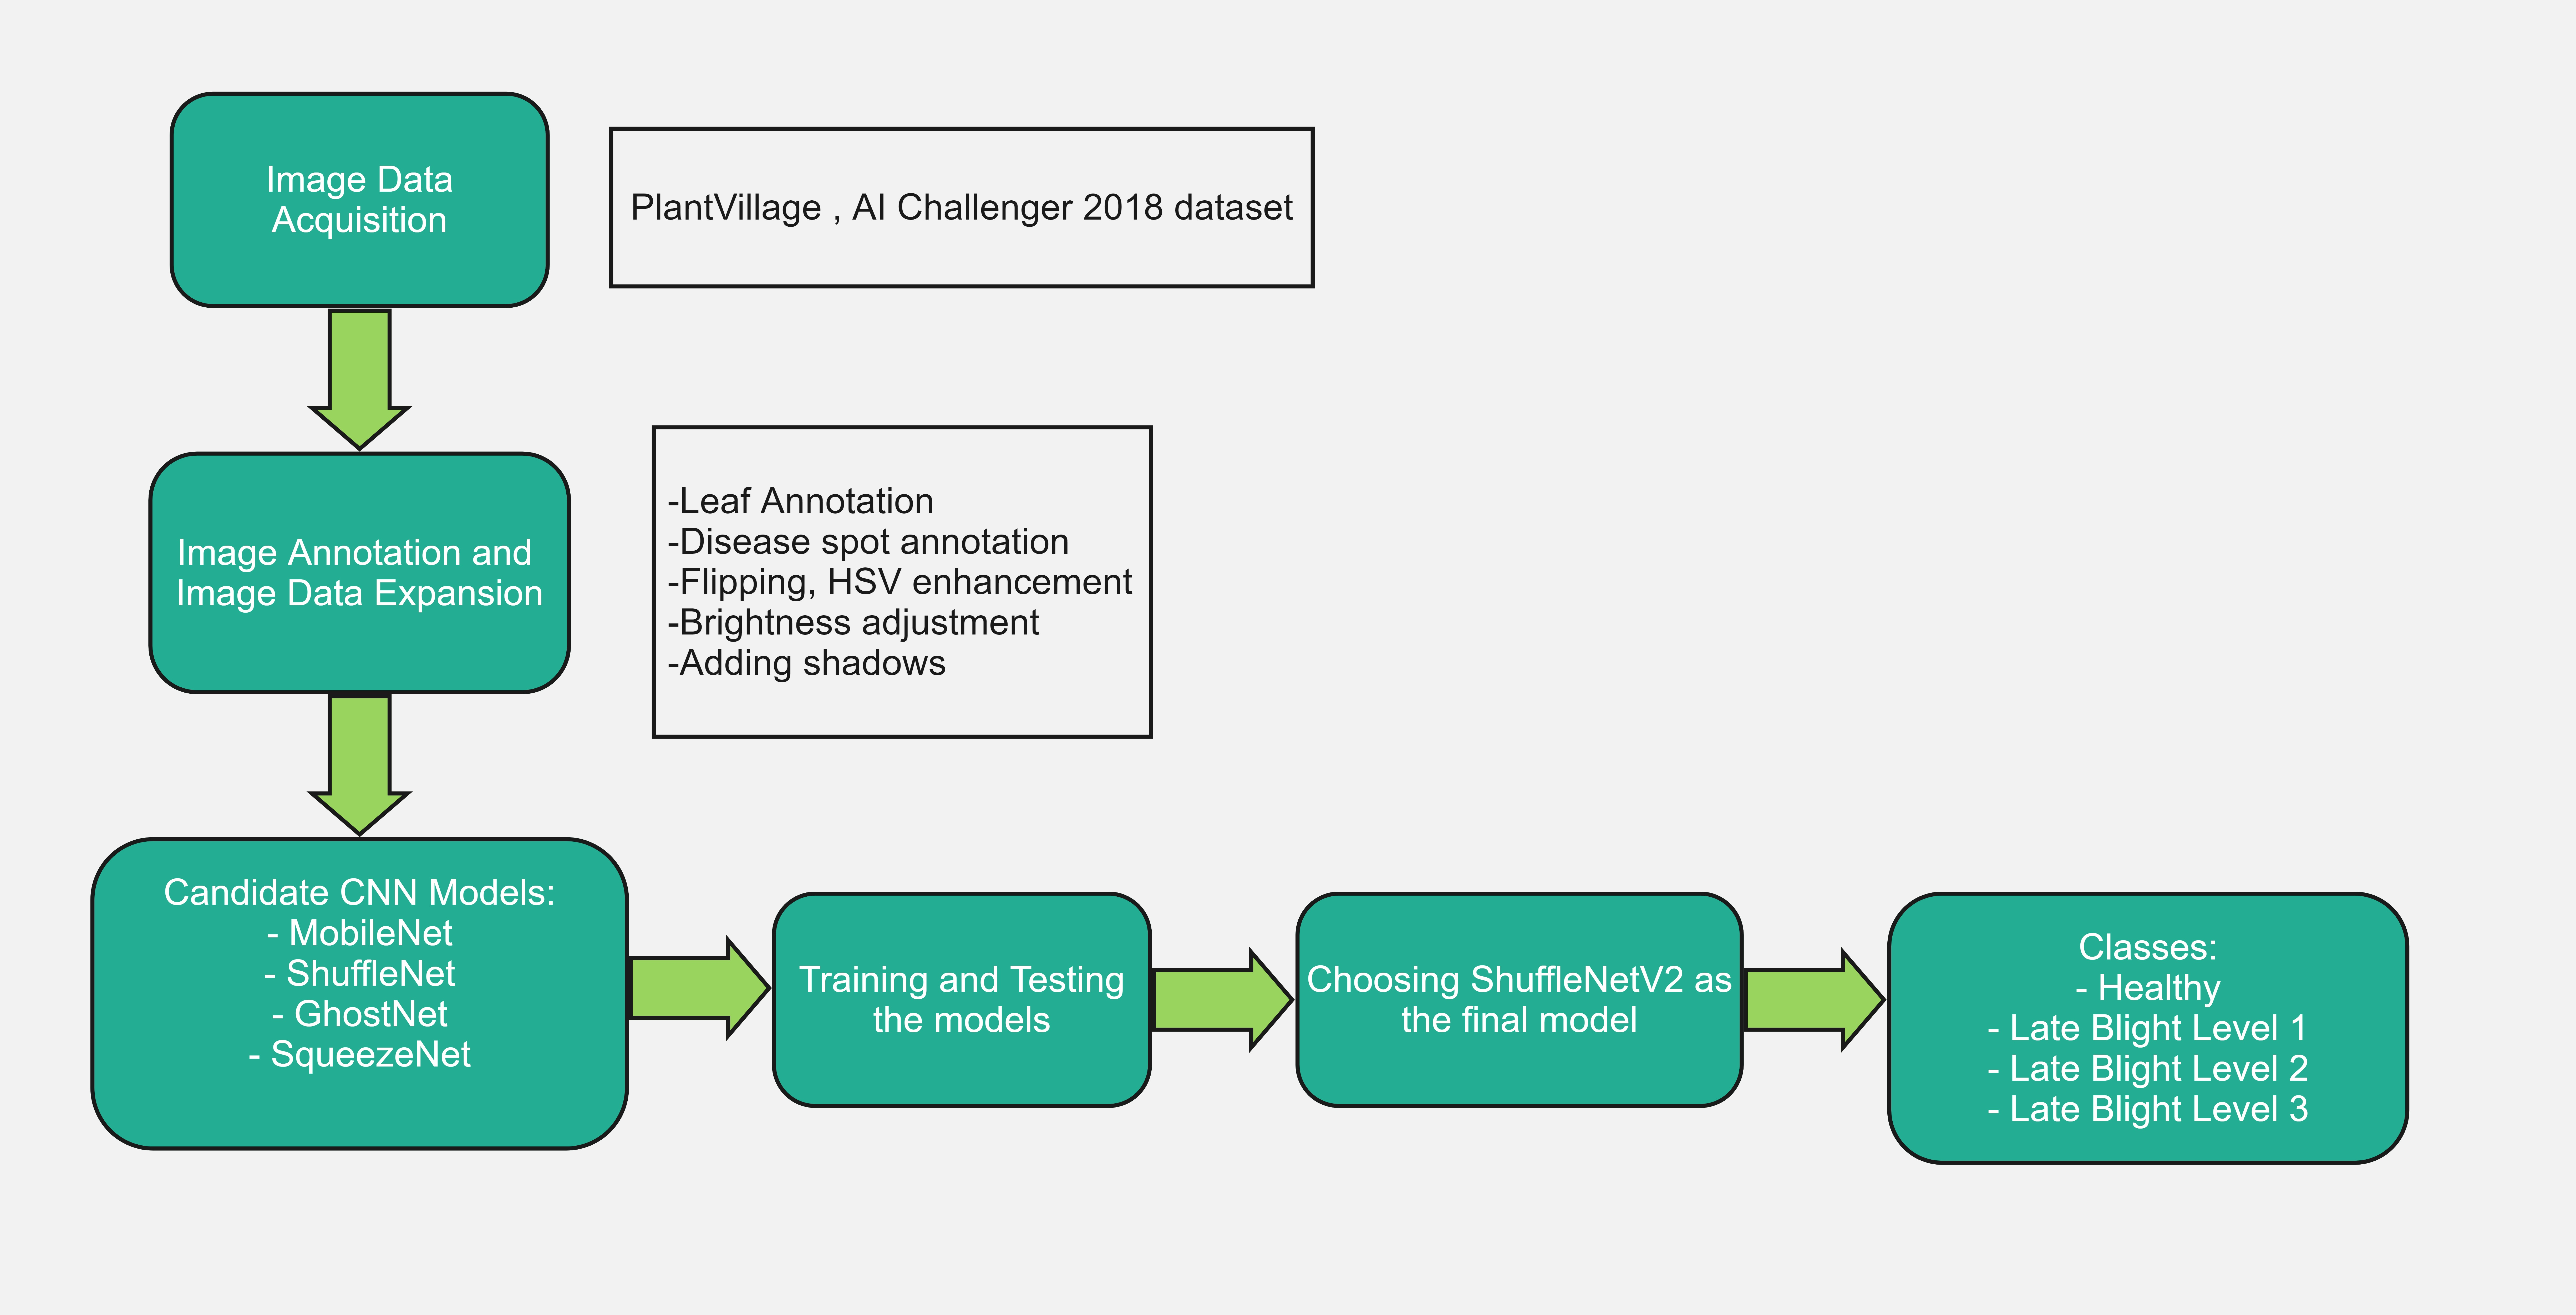
\includegraphics[width=1\textwidth]{2/figures/ant2.2.jpg}
		\caption{Arquitectura del bot de Azure (\cite{antecedente2})}
	\end{center}
\end{figure}
\begin{enumerate}
	\item Se adquirió la base de datos de imágenes del conjunto de datos PlantVillage y IA Challenger 2018 dataset, del cual solo extrajo imágenes de hoja de papa.
	\item Realizaron un preprocesamiento de imágenes donde usaron técnicas para la Anotación de hoja, Zona de enfermedad, Volteo de imagen, Mejora HSV, Ajuste de birllo, Agregar sombras
	\item Los CNN candidatos fueron  MobileNet, ShuffleNet, GhostNet y SqueezeNet
	\item Entrenamiento y testeo de los modelos.
	\item Se eligió ShuffleNetV2 como modelo final
	\item Las clases que el modelo clasificaba son, Hoja de papa sana, Tizón tardio nivel 1, Tizón tardio nivel 2 y Tizón tardio nivel 3
\end{enumerate}

\subsubsection{Resultados obtenidos}
En esta investigacion, se analizaron distintos resultados con diferentes técnicas. Con la técnica final,ShuffleNetV2 , se obtuvieron resultados un accuracy de 95.41\%. Finalmente, se consideró una mejoría para esta técnica, ya que se buscaba el mejor modelo final posible para un dispositivo móvil disminuyendo el tiempo de procesamiento y el costo computacional, tomando esos objetivos en cuenta, se logró un 95.04\%

\begin{figure}[h]						
	\begin{center}
		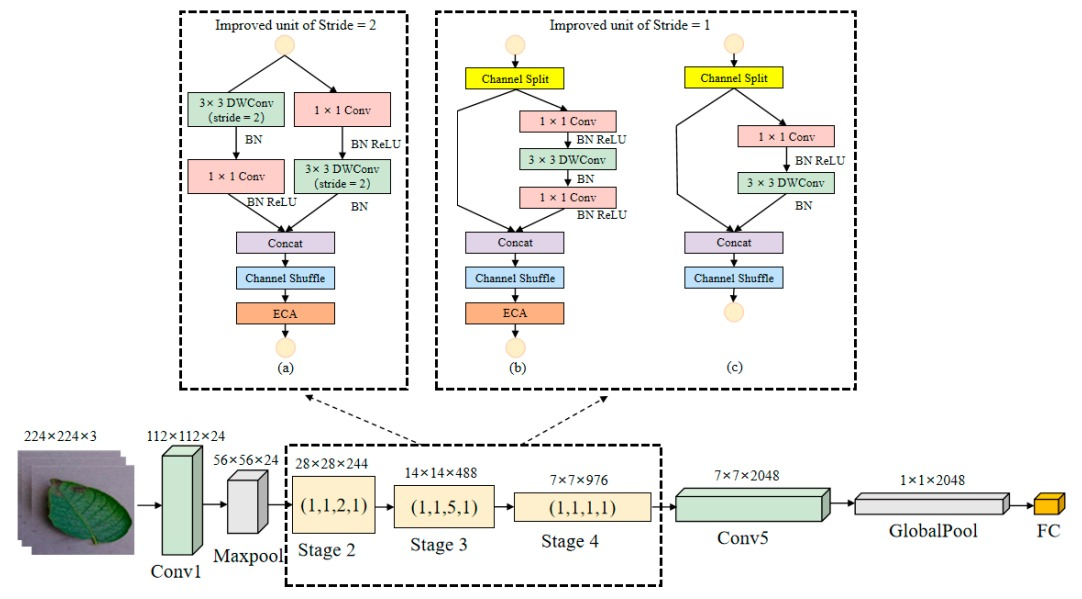
\includegraphics[width=1\textwidth]{2/figures/ant2.3.jpeg}
		\caption{Arquitectura del modelo final. 
			La estructura del modelo mejorado ShuffleNetV2 2×. Nota: La Etapa 2, la Etapa 3 y la Etapa 4 están compuestas por la unidad base original, con Stride = 1, y la unidad modificada está compuesta por una unidad con Stride = 1 y una unidad con Stride = 2. (1, 1, 2, 1) en la Etapa 2 indica una pila de la unidad (a) con Stride = 2 mejorado, una pila de la unidad (b) con Stride = 1 mejorado, dos pilas de la unidad básica con Stride = 1 original, y una pila de la unidad (c) con Stride = 1 mejorado; (1, 1, 5, 1) en la Etapa 3 indica una pila de la unidad (a) con Stride = 2 mejorado, una pila de la unidad (b) con Stride = 1 mejorado, cinco pilas de la unidad básica con Stride = 1 original, y una pila de la unidad (c) con Stride = 1 mejorado; (1, 1, 1, 1) en la Etapa 4 indica una pila de la unidad (a) con Stride = 2 mejorado, una pila de la unidad (b) con Stride = 1 mejorado, una pila de la unidad básica con Stride = 1 original, y una pila de la unidad (c) con Stride = 1 mejorado. (\cite{antecedente2})}
	\end{center}
\end{figure}
\begin{figure}[H]
	\begin{center}
		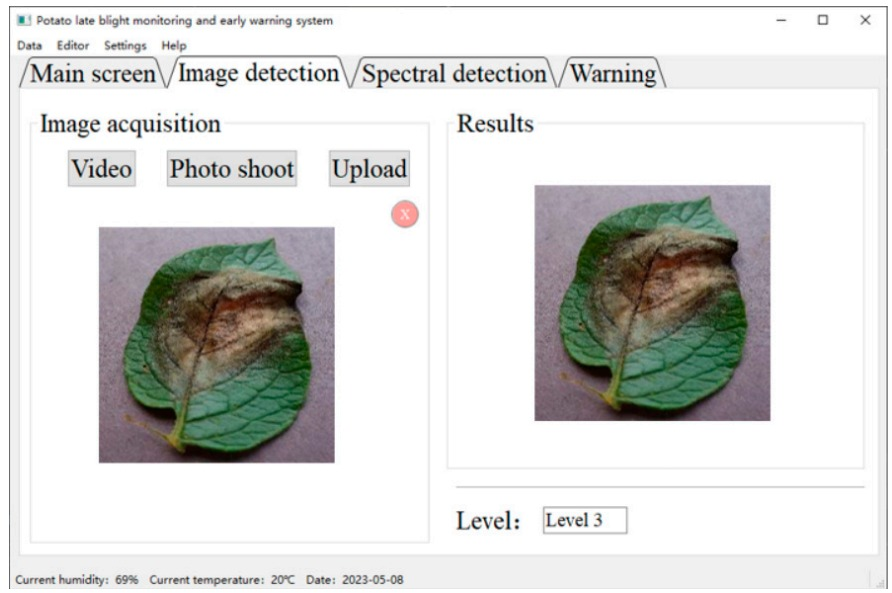
\includegraphics[width=0.7\textwidth]{2/figures/ant2.4.jpeg}
		\caption{Interfaz de operación de detección de imágenes. (\cite{antecedente2})}
	\end{center}
\end{figure}
%%%%%%%%%%%%%%%%%%%%%%%%%%%%%%%%%%%%%%%%%%%%%%%%%%%%%%%%%%%%%%%%%%%%%%%%%%%%%%%%%%%%%%%%%%%%%%%%%%%%%%%%%%%%%%%%%%%%%%%%%%%%


\subsection{Supervised Learning-Based Image Classification for the Detection of Late Blight in Potato Crop \citep*{antecedente3}}

\citeauthor{antecedente3} realizó un trabajo con el fin de ser publicado en la revista Computer Vision and Pattern Recognition Based on Deep Learning. Este fue titulado \citetitle{antecedente3} la cual traducida al español significa  «Clasificación de imágenes basada en aprendizaje supervisado para la detección del tizón tardío en cultivos de papa». La investigación plantea el desarrollo de un modelo de detección temprana del Tizón tardío en la papa utilizando Redes Neuronales Convolucionales y Máquinas de Vectores de Soporte. Asimismo, el autor desarrolló, por sí mismo, su base de datos de imágenes de cultivos de papa. Finalmente, se aplicaron varias métricas de rendimiento, eficiencia y calidad en las tareas de aprendizaje y clasificación para determinar los mejores algoritmos de aprendizaje automático.

\subsubsection{Planteamiento del Problema y objetivo }

La investigación aborda la necesidad de encontrar métodos más eficaces en cuanto a la detección temprana del Tizón Tardío causada por Oomiceto Phytophthora, que afecta rápidamente las hojas, tallos y tubérculos de la papa que es un alimento crucial en la economía de Bógota. Asimismo, la detección tradicional, como pruebas de laboratorio, aunque es eficaz, toma mucho tiempo y es altamente costoso. En conlusión, el objetivo principal del estudio es aplicar técnicas de aprendizaje supervisado y clasificación de imágenes, específicamente mediante redes neuronales convolucionales (CNN) y máquinas de vectores de soporte (SVM), para la detección temprana del tizón tardío en cultivos de papa.

\subsubsection{Fundamento Teórico usado por el Autor}

El autor plantea hacer uso de CNN y SVM como sus posibles modelos finales. Utiliza una CNN, según el preprocesamiento de la data, no modificada y una aumentada, por otro lado, divide SVM en cuatro posibles modelos según caracteristica del preprocesamiento: Color, Textura, PCA, Combined. 

\subsubsection{Metodología empleada por los autores}
La metodología empleada por el autor, para la creación de su modelo consiste en los siguientes pasos: 

\begin{enumerate}
    \item Captura los datos imputados por parte del cliente.
    \item Envía el query a Dialogflow para su procesamiento.
    \item Se procesa la información mediante una API externa y el código implementado, así como la base de datos.
    \item Retorna los resultados procesados y se agrega información extra requerida.
    \item Envía al cliente o usuario la respuesta.
\end{enumerate}

\begin{figure}[H]
	\begin{center}
		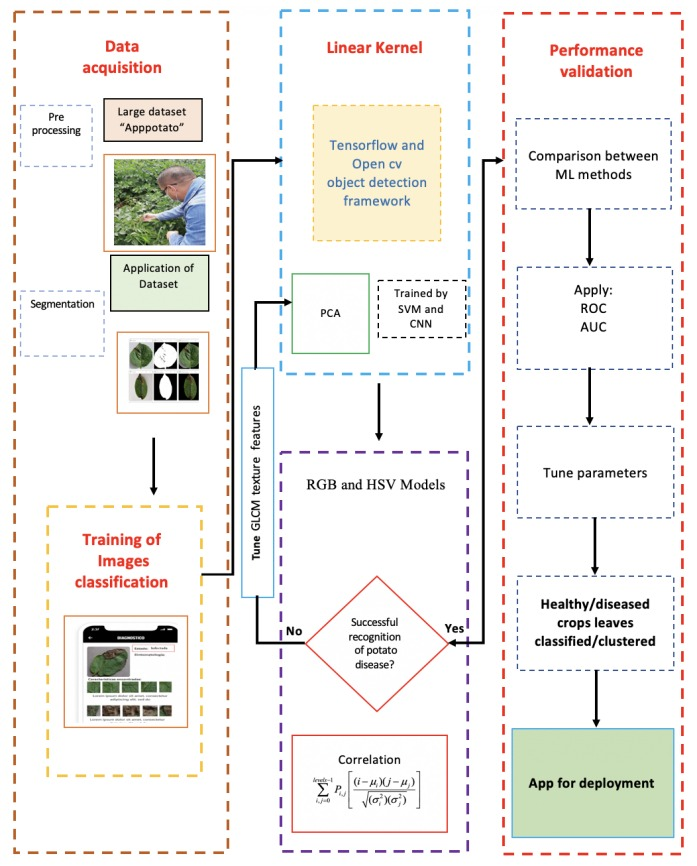
\includegraphics[width=1\textwidth]{2/figures/ant3.jpeg}
		\caption{Diagrama de la metodologia Flowchart(\cite{antecedente3})}
	\end{center}
\end{figure}

\subsubsection{Resultados obtenidos}

Las CNN entrenadas con el conjunto de datos aumentado mostraron el mejor desempeño con una precisión del 93\% y una AUC de 0.97. Además, las SVM entrenadas con características de color obtuvieron mejores resultados en comparación con las SVM entrenadas con otras características. Finalmente, se propone desarrollar una aplicación móvil con características avanzadas para la agricultura de precisión que ayude a los agricultores a identificar la enfermedad del tizón tardío de manera no invasiva y en tiempo real..

%%%%%%%%%%%%%%%%%%%%%%%%%%%%%%%%%%%%%%%%%%%%%%%%%%%%%%%%%%%%%%%%%%%%%%%%%%%%%%%%%%%%%%%%%%%%%%%%%%%%%%%%%%%%%%%%%%%%%%%%%%%%
\subsection{Potato Blight Classification Android Application using Deep Learning  \citep*{antecedente5}}

\citeauthor{antecedente5} realizó un artículo publicado en base de datos de ELSEVIER, siendo también parte de la revista Sustainable Chemistry and Pharmacy en el año 2022. Este fue titulado \citetitle{antecedente5} la cual traducida al español significa «Redes neuronales convolucionales profundas para la detección de enfermedades de la hoja del tomate basada en imágenes». El trabajo nos dice que el reconocimiento de enfermedades foliares en las plantas representa un riesgo significativo para la seguridad alimentaria, ya que puede reducir la producción agrícola y, por ende, la economía nacional. Es crucial identificar estas enfermedades en etapas tempranas para mejorar la calidad y cantidad de los productos agrícolas. Por lo tanto, se requiere un sistema automático de reconocimiento de enfermedades foliares que pueda identificar y clasificar estas enfermedades en etapas tempranas. En este contexto, se han utilizado modelos de redes neuronales convolucionales profundas (DCNN) para el análisis de imágenes de hojas, con el objetivo de mejorar la precisión y reducir el tiempo de respuesta en la identificación de enfermedades foliares en tomates. Se propone un sistema automático de identificación de enfermedades foliares en tomates utilizando DCNN, con un conjunto de datos de 18160 imágenes de hojas de tomate. Este conjunto de datos se dividió en un 60\% para entrenamiento y un 40\% para pruebas, logrando una precisión del 98.40\% en el conjunto de pruebas con el modelo DCNN propuesto.

\subsubsection{Planteamiento del Problema y objetivo }

El artículo aborda principalmente que las enfermedades en las hojas de tomate causan pérdidas significativas en la producción, afectando tanto la calidad como la cantidad de los productos. Identificar y diagnosticar estas enfermedades de manera temprana es crucial, ya que pueden reducir drásticamente el crecimiento de los cultivos y, por lo tanto, la producción. Sin embargo, el diagnóstico manual de las enfermedades foliares puede llevar a una disminución en la producción debido a la gravedad de las enfermedades y a la variabilidad en los síntomas causada por factores ambientales como la temperatura, el viento y la humedad. Por lo tanto, existe una necesidad de desarrollar un sistema automático que pueda identificar y diagnosticar estas enfermedades en etapas tempranas, permitiendo a los agricultores tomar medidas preventivas adecuadas para proteger sus cultivos. El objetivo es desarrollar una herramienta automática que diagnostique las enfermedades de las hojas de tomate tempranamente para mejorar la producción agrícola. Se utilizará un enfoque basado en redes neuronales convolucionales profundas (DCNN) para clasificar 10 tipos de enfermedades en los cultivos de tomate, con el fin de identificar los síntomas de las hojas en etapas tempranas y mejorar la eficiencia y precisión del modelo mediante técnicas de ajuste de parámetros.

\subsubsection{Fundamento Teórico usado por el Autor}

Los autores plantean utilizar como técnica principal una DCNN (Deep Convolutional Neural Networks) y compararla con técnicas como MLP (Multiplayer Layer Perceptron) y SVM (Support Vector Machine).



\subsubsection{Metodología empleada por los autores}
La metodología empleada por los autores, para la creación de su chatbot consiste en los siguientes pasos: 

\begin{figure}[H]
	\begin{center}
		
\includegraphics[width=1\textwidth]{2/figures/ant5.jpg}
		\caption{Metodología (\cite{antecedente5})}
	\end{center}
\end{figure}

\subsubsection{Resultados obtenidos}
Como resultado del desarrollo del modelo final, este alcanzó un 98.40\% de accuracy promedio, mientras que SVM obtuvo un accuracy de 90.01\% y MLP un accuracy de 88.30\%. 

\begin{figure}[H]
	\begin{center}
		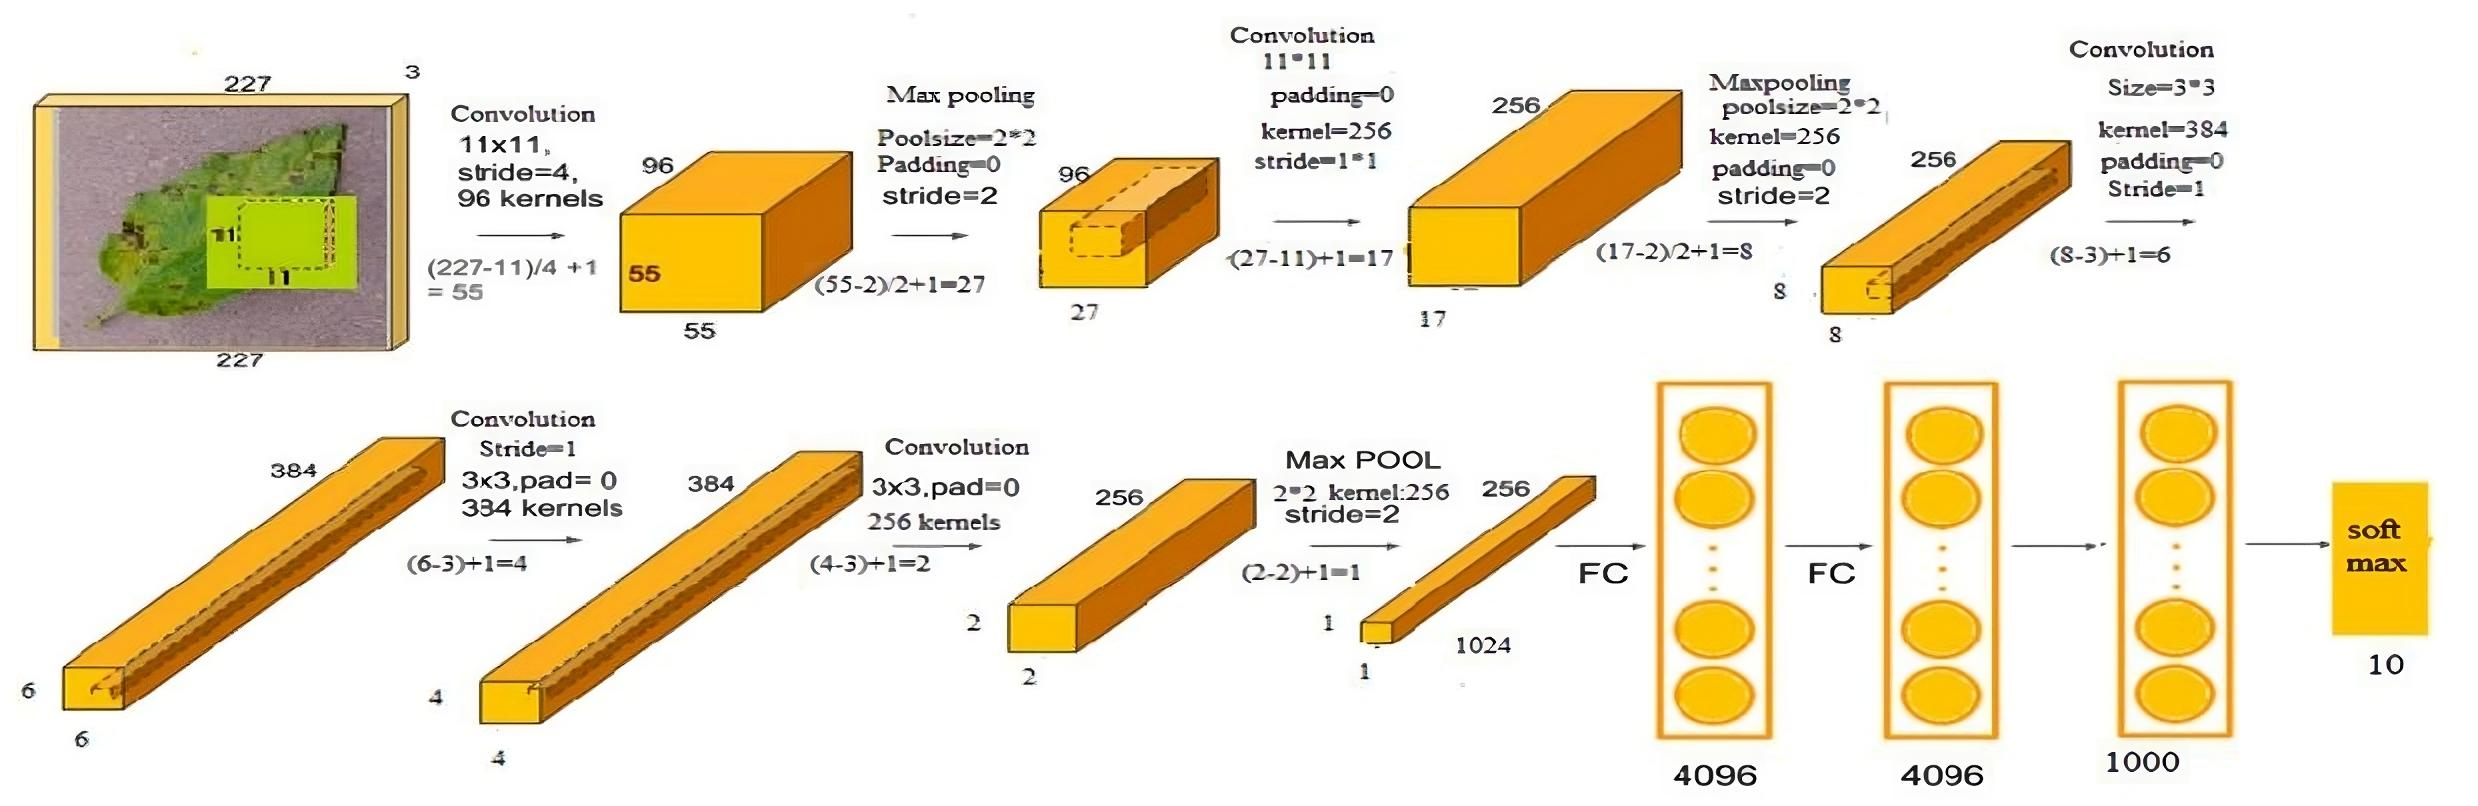
\includegraphics[width=1\textwidth]{2/figures/ant5.2.jpeg}
		\caption{Arquitectura del modelo final (\cite{antecedente5})}
	\end{center}
\end{figure}
%%%%%%%%%%%%%%%%%%%%%%%%%%%%%%%%%%%%%%%%%%%%%%%%%%%%%%%%%%%%%%%%%%%%%%%%%%%%%%%%%%%%%%%%%%%
%%%%%%%%%%%%%%%%%%%%%%%%%%%%%%%%%%%%%%%%%%%%%%%%%%%%%%%%%%%%
\subsection{Deep Convolutional Neural Networks for image based tomato leaf disease detection  \citep*{antecedente6}}

\citeauthor{antecedente6} realizó un artículo publicado en base de datos de International Journal of Advanced Research in Science, Communication and Technology (IJARSCT) en el año 2023. Este fue titulado \citetitle{antecedente6} la cual traducida al español significa «Aplicación para Android de clasificación del tizón de la papa usando el aprendizaje profundo». La investigación sostiene que los agricultores de papas sufren pérdidas económicas debido a enfermedades como el tizón temprano y tardío. La detección temprana y tratamiento adecuado pueden prevenir estas pérdidas, pero los métodos tradicionales son lentos y propensos a errores. Proponemos usar una Red Neuronal Convolucional (CNN) personalizada para diagnosticar enfermedades de plantas de manera rápida y precisa, reduciendo el tiempo de computación y minimizando errores, lo que ayuda a los agricultores a tratar las enfermedades a tiempo y reducir pérdidas.

\subsubsection{Planteamiento del Problema y objetivo }
El trabajo sustenta que la industria de la papa enfrenta un desafío significativo en la prevención de pérdidas de cultivos debido a enfermedades como el tizón temprano y el tizón tardío. Estas enfermedades pueden causar pérdidas económicas sustanciales para los agricultores si no se detectan y tratan a tiempo. Los métodos tradicionales de inspección visual son lentos, propensos a errores y no son viables para aplicaciones en tiempo real debido a los largos tiempos de procesamiento de imágenes. Además, existe la necesidad de mejorar la precisión y reducir el tiempo de computación en los métodos actuales de diagnóstico de enfermedades de las plantas. Por eso, su objetivo es desarrollar una red neuronal convolucional (CNN) eficiente y precisa para detectar enfermedades en las plantas de papa, reduciendo el tiempo de computación y mejorando la precisión, con el fin de ayudar a los agricultores a tratar las enfermedades a tiempo y reducir pérdidas económicas. 

\subsubsection{Fundamento Teórico usado por el Autor}

Los autores formulan utilizar como técnica principal un Red Neuronal Convolucional, mejorarla para que sea una Red neuronal convolucional personalizada de enfermedades profundas (PDDCNN), ya que buscan lograr un modelo que se adapte a distintas regiones de donde se pueda obtener el dataset.


\subsubsection{Metodología empleada por los autores}
La metodología empleada por los autores, para la creación de su chatbot consiste en los siguientes pasos: 

\begin{figure}[H]
	\begin{center}
		
\includegraphics[width=1\textwidth]{2/figures/ant6.jpg}
		\caption{Metodología (\cite{antecedente6})}
	\end{center}
\end{figure}

\subsubsection{Resultados obtenidos}
Los resultados finales fueron tomados sobre la base de datos que ellos crearon después de entrenar su modelo con el conjunto de datos PlantVillage. Obtuvo un accuracy de 99\% en el tizon tardio y tizon temprano, mientras que en las hojas sanas tuvieron un accuracy de 100\% 

\begin{figure}[H]
	\begin{center}
		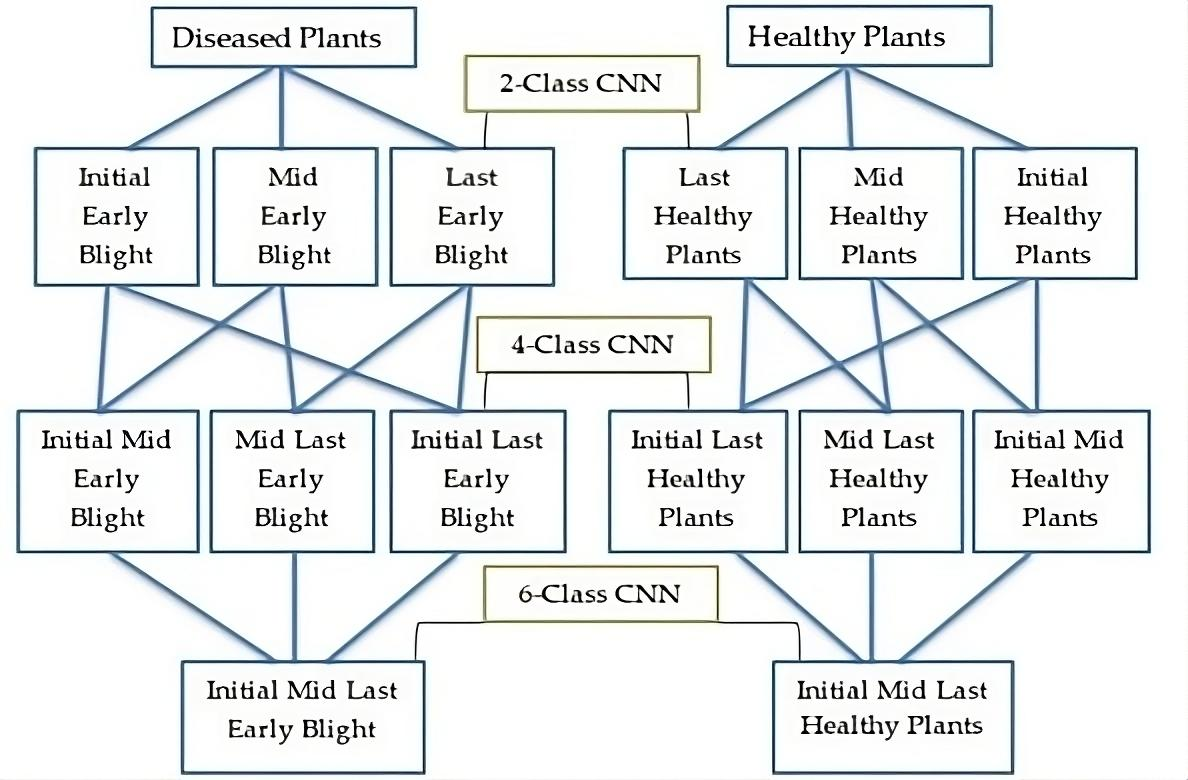
\includegraphics[width=1\textwidth]{2/figures/ant6.2.jpeg}
		\caption{Arquitectura del modelo final (\cite{antecedente6})}
	\end{center}
\end{figure}
%%%%%%%%%%%%%%%%%%%%%%%%%%%%%%%%%%%%%%%%%%%%%%%%%%%%%%%%%%%%%%%%%%%%%%%%%%%%%%%%%%%%%%%%%%%%%%%%%%%%%%%%%%%%%%%%%%%%%%%%%%%%%%
\subsection{Potato Blight Classification Android Application using Deep Learning  \citep*{antecedente7}}

\citeauthor{antecedente7} realizó un artículo publicado en base de datos de ELSEVIER, siendo también parte de la revista Sustainable Chemistry and Pharmacy en el año 2022. Este fue titulado \citetitle{antecedente7} la cual traducida al español significa «Redes neuronales convolucionales profundas para la detección de enfermedades de la hoja del tomate basada en imágenes». El trabajo nos dice que el reconocimiento de enfermedades foliares en las plantas representa un riesgo significativo para la seguridad alimentaria, ya que puede reducir la producción agrícola y, por ende, la economía nacional. Es crucial identificar estas enfermedades en etapas tempranas para mejorar la calidad y cantidad de los productos agrícolas. Por lo tanto, se requiere un sistema automático de reconocimiento de enfermedades foliares que pueda identificar y clasificar estas enfermedades en etapas tempranas. En este contexto, se han utilizado modelos de redes neuronales convolucionales profundas (DCNN) para el análisis de imágenes de hojas, con el objetivo de mejorar la precisión y reducir el tiempo de respuesta en la identificación de enfermedades foliares en tomates. Se propone un sistema automático de identificación de enfermedades foliares en tomates utilizando DCNN, con un conjunto de datos de 18160 imágenes de hojas de tomate. Este conjunto de datos se dividió en un 60\% para entrenamiento y un 40\% para pruebas, logrando una precisión del 98.40\% en el conjunto de pruebas con el modelo DCNN propuesto.

\subsubsection{Planteamiento del Problema y objetivo }

El artículo aborda principalmente que las enfermedades en las hojas de tomate causan pérdidas significativas en la producción, afectando tanto la calidad como la cantidad de los productos. Identificar y diagnosticar estas enfermedades de manera temprana es crucial, ya que pueden reducir drásticamente el crecimiento de los cultivos y, por lo tanto, la producción. Sin embargo, el diagnóstico manual de las enfermedades foliares puede llevar a una disminución en la producción debido a la gravedad de las enfermedades y a la variabilidad en los síntomas causada por factores ambientales como la temperatura, el viento y la humedad. Por lo tanto, existe una necesidad de desarrollar un sistema automático que pueda identificar y diagnosticar estas enfermedades en etapas tempranas, permitiendo a los agricultores tomar medidas preventivas adecuadas para proteger sus cultivos. El objetivo es desarrollar una herramienta automática que diagnostique las enfermedades de las hojas de tomate tempranamente para mejorar la producción agrícola. Se utilizará un enfoque basado en redes neuronales convolucionales profundas (DCNN) para clasificar 10 tipos de enfermedades en los cultivos de tomate, con el fin de identificar los síntomas de las hojas en etapas tempranas y mejorar la eficiencia y precisión del modelo mediante técnicas de ajuste de parámetros.

\subsubsection{Fundamento Teórico usado por el Autor}

Los autores plantean utilizar como técnica principal una DCNN (Deep Convolutional Neural Networks) y compararla con técnicas como MLP (Multiplayer Layer Perceptron) y SVM (Support Vector Machine).

\subsubsection{Metodología empleada por los autores}
La metodología empleada por los autores, para la creación de su modelo consiste en los siguientes pasos: 

\begin{figure}[H]
	\begin{center}
		
\includegraphics[width=1\textwidth]{2/figures/ant7.jpg}
		\caption{Metodología (\cite{antecedente7})}
	\end{center}
\end{figure}

\subsubsection{Resultados obtenidos}
Para escoger su modelo consideraron VGG19 con la técnica de clasificación Logistic Regresion. Este alcanzó 97.8\% de accuracy sobre el testeo del dataset. 

\begin{figure}[H]
	\begin{center}
		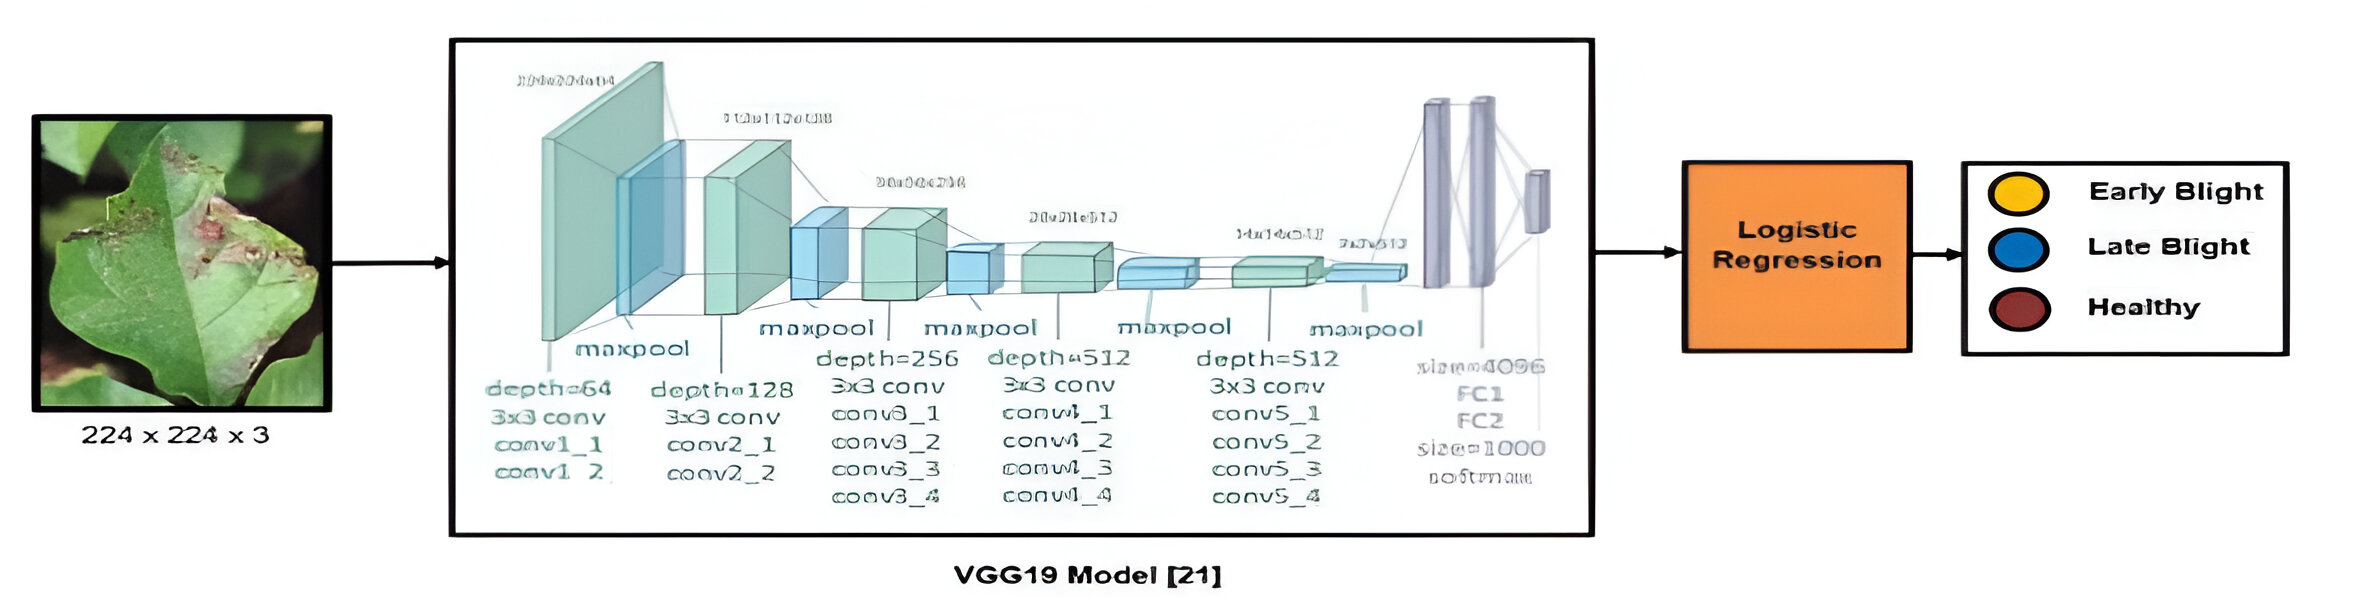
\includegraphics[width=1\textwidth]{2/figures/ant7.2.jpeg}
		\caption{Arquitectura del modelo final (\cite{antecedente7})}
	\end{center}
\end{figure}
%%%%%%%%%%%%%%%%%%%%%%%%%%%%%%%%%%%%%%%%%%%%%%%%%%%%%%%%%%%%%%%%%%%%%%%%%%%%%%%%%%%%%%%%%%%%%%%%%%%%%%%%%%%%%%%%%%%%%%%%%%%%%%
\subsection{Investigation of Phytophthora Infestans Causing Potato Late Blight Disease: A Review \citep*{antecedente4}}

\citeauthor{antecedente4} realizó un trabajo con el fin de ser publicado en la revista Biomedicine and Chemical Sciences. Este fue titulado \citetitle{antecedente4} la cual traducida al español significa  «Investigación de Phytophthora Infestans que causa el tizón tardío de la papa». La investigación sostiene Phytophthora infestans causa el tizón tardío de la papa, infectando raíces, tubérculos y brotes. La propagación se debe al cultivo de tubérculos infectados y restos de plantas en el campo. Las estructuras como micelio, zoosporas, oosporas y esporangios pueden causar infección, y las oosporas pueden sobrevivir de 3 a 4 años en bajas temperaturas. P. infestans puede causar pérdidas de hasta el 100\% en condiciones óptimas. Hay dos patrones de apareamiento, A1 y A2, y varios patrones genéticos que complican el control de la enfermedad. Las estrategias de control incluyen químicos, rotación de cultivos, agentes biológicos y plantas resistentes, siendo más efectivo combinar plantas resistentes y fungicidas. El artículo analiza los factores de propagación y desafíos del tizón tardío.
\subsubsection{Planteamiento del Problema y objetivo }

La investigación aborda que el hongo Phytophthora sp, con más de 60-80 especies, infecta diversas plantas, incluidas las papas y los tomates. Phytophthora infestans, en particular, causa estragos en estos cultivos, provocando pérdidas significativas de rendimiento y desencadenando eventos históricos como la hambruna irlandesa en la década de 1840. A pesar de los esfuerzos de control, la enfermedad del tizón tardío sigue siendo una amenaza global para la producción de papas, con pérdidas que pueden variar del 50 al 100\% dependiendo de diversos factores ambientales y de gestión. El objetivo principal es investigar Phytophthora infestans y su impacto en la enfermedad del tizón tardío en las papas. Se busca comprender mejor los modos de infección, las estrategias de reproducción del patógeno y los factores que contribuyen a su agresividad. A través de esta investigación, se espera identificar mejores métodos de control y gestión de la enfermedad, incluyendo el uso de fungicidas, prácticas culturales y la resistencia de las plantas hospederas, para mitigar las pérdidas económicas y asegurar la seguridad alimentaria en las regiones afectadas.

\subsubsection{Fundamento Teórico usado por el Autor}

El autor desarrolla su investigación en base a múltiples investigaciones pasadas. Desde los orígenes del Tizón tardío, hasta su condición en el mundo actual.

\subsubsection{Metodología empleada por los autores}
La metodología empleada por el autor, para la creación de su chatbot consiste en los siguientes pasos: 


\begin{figure}[H]
	\begin{center}
		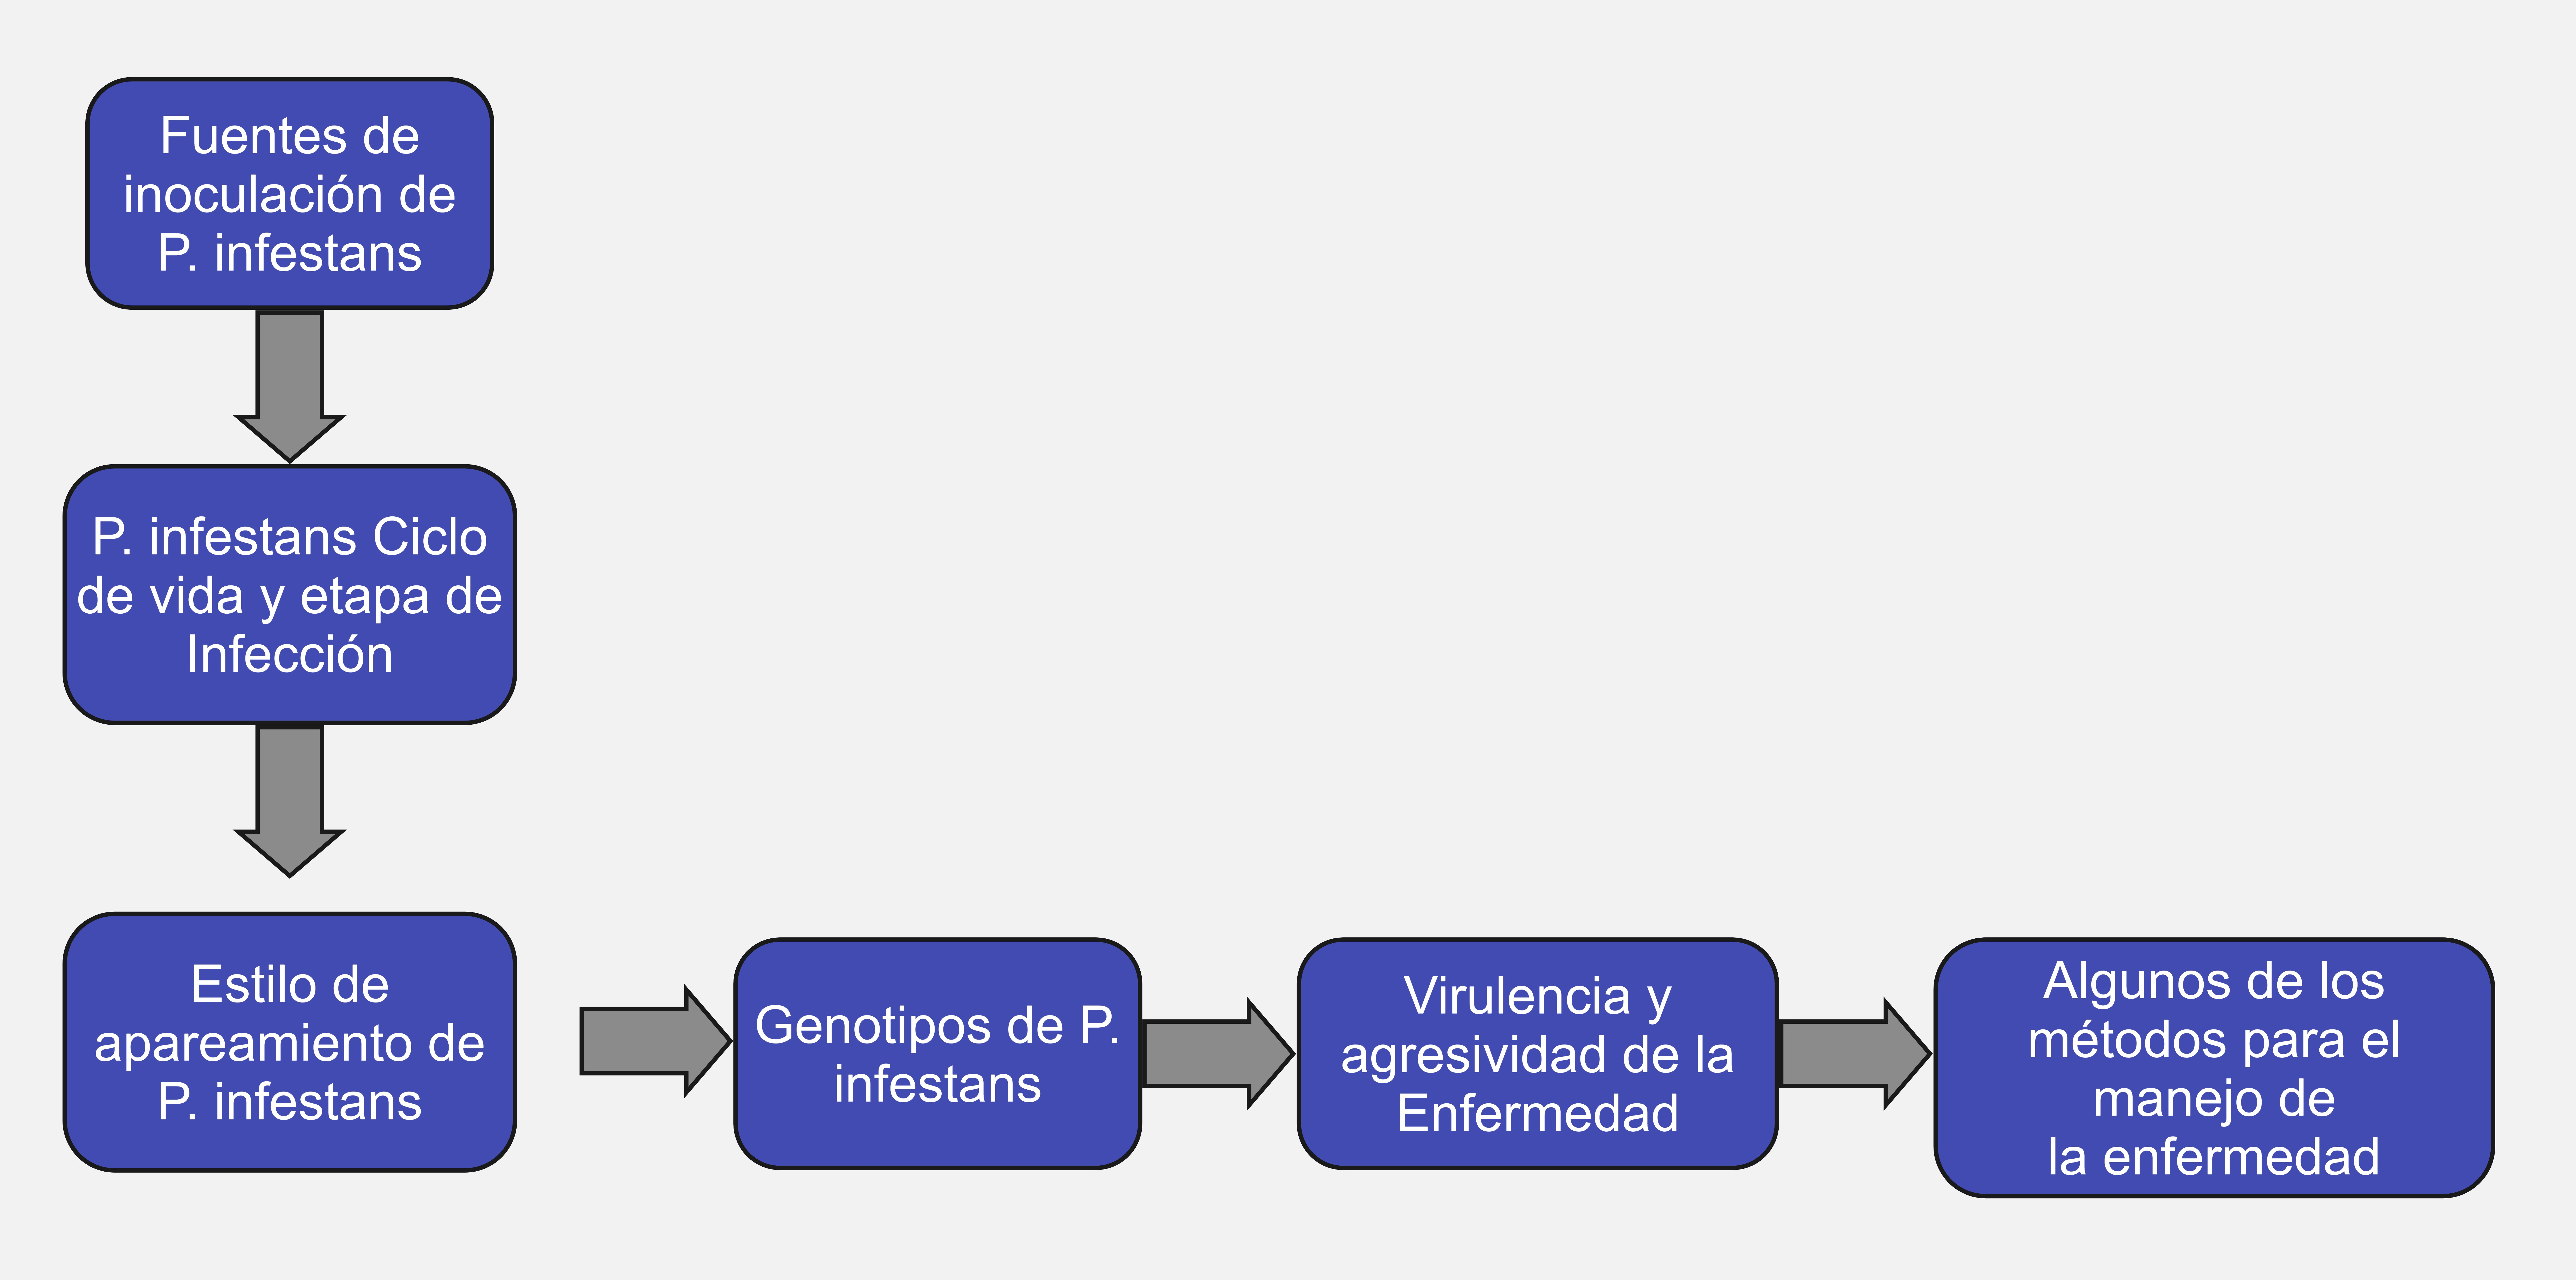
\includegraphics[width=1\textwidth]{2/figures/ant4.jpg}
		\caption{Diagrama de la metodologia(\cite{antecedente4})}
	\end{center}
\end{figure}

\subsubsection{Resultados obtenidos}

Los aislamientos de P. infestans tienen varias estructuras de infección que pueden infectar diferentes partes de la planta de papa y pueden sobrevivir durante un largo período. El hongo es capaz de reproducirse tanto sexual como asexualmente, y también presenta patrones de apareamiento A1 y A2 y diferentes genotipos. Todas estas características han llevado a la aparición de varios desafíos en el estudio de la virulencia y la agresividad. El segundo y más importante desafío incluye cómo elegir el mejor método para controlar la enfermedad (tizón tardío), ya que aparecen aislamientos que pueden resistir diferentes fungicidas, también pueden infectar plantas resistentes y muchas razones hacen que este desafío sea más importante.

%%%%%%%%%%%%%%%%%%%%%%%%%%%%%%%%%%%%%%%%%%%%%%%%%%%%%%%%%%%%%%%%%%%%%%%%%%%%%%%%%%%%%%%%%%%%%%%%%%%%%%%%%%%%%%%%%%%%%%%%%%%%




%%%%%%%%%%%%%%%%%%%%%%%%%%%%%%%%%%%%%%%%%%%%%%%%%%%%%%%%%%%%%%%%%%%%%%%%%%%%%%%%%%%%%%%%%%%%%%%%%%%%%%%%%%%%%%%%%%%%%%%%%%%%

%%%%%%%%%%%%%%%%%%%%%%%%%%%%%%%%%%%%%%%%%%%%%%%%%%%%%%%%%%%%%%%%%%%%%%%%%%%%%%%%%%%%%%%%%%%%%%%%%%%%%%%%%%%%%%%%%%%%%%%%%%%%

%%%%%%%%%%%%%%%%%%%%%%%%%%%%%%%%%%%%%%%%%%%%%%%%%%%%%%%%%%%%%%%%%%%%%%%%%%%%%%%%%%%%%%%%%%%%%%%%%%%%%%%%%%%%%%%%%%%%%%%%%%%%

%%%%%%%%%%%%%%%%%%%%%%%%%%%%%%%%%%%%%%%%%%%%%%%%%%%%%%%%%%%%%%%%%%%%%%%%%%%%%%%%%%%%%%%%%%%%%%%%%%%%%%%%%%%%%%%%%%%%%%%%%%%%

%%%%%%%%%%%%%%%%%%%%%%%%%%%%%%%%%%%%%%%%%%%%%%%%%%%%%%%%%%%%%%%%%%%%%%%%%%%%%%%%%%%%%%%%%%%%%%%%%%%%%%%%%%%%%%%%%%%%%%%%%%%%

% %%%Ecuacion
% \begin{equation}  
% \label{eq:RMSE}
% RMSE = \sqrt{\frac{\sum_{i=1}^{N}{\Big(O_i -T_i\Big)^2}}{N}}
% \end{equation}